\chapter{Eksperymenty i wyniki (część badawcza)}

W niniejszym rozdziale przedstawiono przebieg oraz wyniki eksperymentów przeprowadzonych w celu oceny zdolności modeli uczenia maszynowego do pasywnej estymacji funkcjonalnego progu mocy (FTP). Szczególną uwagę poświęcono identyfikacji wycieku danych wynikającego z bezpośredniego powiązania części cech wejściowych ze zmienną celu.

\section{Charakterystyka przygotowanego zbioru danych}

Po kontrolowanym przetwarzaniu wykorzystano dane z 781 archiwów ZIP ze zbioru GoldenCheetah OpenData. Zastosowano filtr wartości etykiety FTP: do eksperymentu dopuszczono wyłącznie sesje spełniające warunek $50 \le \mathrm{ftp\_label} \le 500\ \mathrm{W}$. Pozwoliło to odrzucić skrajne wartości odstające, które mogły wynikać z artefaktów lub błędów pomiarowych.

Finalny plik eksperymentalny obejmował 726 zawodników oraz 151\,399 sesji treningowych. Zmienną celu stanowiła wartość \texttt{ftp\_label}. Strukturę przygotowanego zbioru przedstawiono w tabeli~\ref{tab:struktura_zbioru}.

Liczba sesji jest istotna z punktu widzenia uczenia modeli, ale nie oznacza pełnej niezależności obserwacji. Jeden zawodnik może dostarczać wiele aktywności realizowanych w różnych okresach. Z tego względu liczby rekordów nie należy utożsamiać z liczbą niezależnych osób. Właściwym zabezpieczeniem metodologicznym jest podział osobniczy opisany w kolejnej sekcji.

\begin{table}[htbp]
\centering
\caption{Struktura przygotowanego zbioru danych wykorzystanego w eksperymentach}
\label{tab:struktura_zbioru}
\small
\begin{tabular}{|>{\raggedright\arraybackslash}p{4.4cm}|>{\raggedright\arraybackslash}p{9.4cm}|}
\hline
\textbf{Element struktury} & \textbf{Charakterystyka} \\ \hline
Źródło danych & Zanonimizowane sesje telemetryczne na podstawie 781 archiwów ZIP GoldenCheetah OpenData \\ \hline
Liczba zawodników & 726 \\ \hline
Liczba obserwacji przed filtrem & 152\,010 sesji treningowych \\ \hline
Liczba obserwacji po filtrze & 151\,399 sesji treningowych \\ \hline
Liczba odrzuconych wartości odstających & 611 sesji treningowych \\ \hline
Zakres filtra FTP & $50 \le \mathrm{ftp\_label} \le 500\ \mathrm{W}$ \\ \hline
Zmienna celu & \texttt{ftp\_label} \\ \hline
Liczba cech wariantu B & 46 \\ \hline
Liczba cech wariantu C & 41 \\ \hline
\end{tabular}
\par\smallskip
\raggedright\footnotesize Źródło: Opracowanie własne na podstawie przetworzonych danych GoldenCheetah OpenData.
\end{table}

\FloatBarrier
\section{Konfiguracja eksperymentu i podział danych}

Zastosowano podział osobniczy (ang.\ \textit{subject-wise split}) z wykorzystaniem mechanizmu \texttt{GroupShuffleSplit}. Identyfikator \texttt{athlete\_id} pełnił rolę zmiennej grupującej, dzięki czemu wszystkie sesje danego zawodnika trafiały wyłącznie do jednego podzbioru. Test odbywał się zatem na zawodnikach nieobecnych w zbiorze treningowym.

Podział wykonano z parametrami \texttt{test\_size=0.2} oraz \texttt{random\_state=42}. Szczegółowe podsumowanie przedstawiono w tabeli~\ref{tab:podzial_danych}.

Stała wartość \texttt{random\_state} umożliwia odtworzenie przyjętego podziału. Finalna ocena dotyczy pojedynczego zbioru treningowego i testowego, a nie walidacji krzyżowej. Wyniki należy zatem interpretować jako rezultat konkretnej, jawnie zdefiniowanej ewaluacji historycznej. Podział po zawodniku ogranicza ryzyko zawyżenia metryk przez obecność sesji tej samej osoby po obu stronach eksperymentu.

\begin{table}[htbp]
\centering
\caption{Podział danych na zbiór treningowy i testowy}
\label{tab:podzial_danych}
\small
\begin{tabular}{|>{\raggedright\arraybackslash}p{4.4cm}|>{\raggedright\arraybackslash}p{9.4cm}|}
\hline
\textbf{Parametr} & \textbf{Wartość} \\ \hline
Metoda podziału & \texttt{GroupShuffleSplit} (grupowanie po \texttt{athlete\_id}) \\ \hline
Liczba rekordów (Train) & 117\,903 \\ \hline
Liczba rekordów (Test) & 33\,496 \\ \hline
Proporcja (Test Size) & 0,2 (20\%) \\ \hline
\end{tabular}
\par\smallskip
\raggedright\footnotesize Źródło: Opracowanie własne na podstawie przetworzonych danych GoldenCheetah OpenData.
\end{table}

Porównano trzy warianty predyktorów:
\begin{itemize}
    \item \textbf{Wariant A (kontrolny z wyciekiem danych):} zawierał cechę \texttt{mmp\_20min}, z której wyliczana była etykieta \texttt{ftp\_label}. Wariant służył wyłącznie diagnozie skutków wycieku informacji.
    \item \textbf{Wariant B (główny wariant badawczy):} zawierał 46 cech po usunięciu \texttt{mmp\_20min}.
    \item \textbf{Wariant C (konserwatywny):} zawierał 41 cech po usunięciu wszystkich predyktorów z prefiksem \texttt{mmp\_}.
\end{itemize}

\FloatBarrier
\section{Przebieg eksperymentów, modele i parametry}

Na każdym z wariantów A, B i C uruchomiono trzy algorytmy regresyjne: Ridge Regression, Random Forest oraz XGBoost. Ridge Regression stanowił liniowy punkt odniesienia. Random Forest agregował predykcje wielu drzew decyzyjnych, natomiast XGBoost reprezentował rodzinę modeli Gradient Boosting, w których kolejne drzewa korygują błędy wcześniejszych elementów.

Porównanie trzech klas modeli umożliwia ocenę, czy w danych dominuje zależność możliwa do przybliżenia liniowo, czy też dodatkową wartość przynoszą algorytmy odwzorowujące nieliniowości i interakcje cech. Ridge Regression jest celowo prostym punktem odniesienia: po standaryzacji predyktorów dopasowuje liniową relację regularyzowaną karą $\ell_2$. Random Forest zmniejsza wariancję pojedynczego drzewa przez agregację wielu modeli budowanych na losowanych danych i podzbiorach cech. XGBoost uczy kolejne drzewa sekwencyjnie, kierując je na błędy pozostawione przez wcześniejsze elementy zespołu.

Konfigurację modeli przedstawiono w tabeli~\ref{tab:konfiguracja_modeli}. Dla każdego modelu obliczono metryki MAE, RMSE, $R^2$ oraz MedAE na tym samym zbiorze testowym. MAE i MedAE opisują typową wielkość błędu w watach, RMSE silniej uwzględnia większe pomyłki, a $R^2$ informuje o części wariancji etykiety wyjaśnianej przez model.

\begin{table}[htbp]
\centering
\caption{Konfiguracja modeli wykorzystanych w eksperymencie}
\label{tab:konfiguracja_modeli}
\small
\begin{tabular}{|>{\raggedright\arraybackslash}p{2.8cm}|>{\raggedright\arraybackslash}p{3.8cm}|>{\raggedright\arraybackslash}p{6.8cm}|}
\hline
\textbf{Model} & \textbf{Przetwarzanie wstępne} & \textbf{Najważniejsze parametry} \\ \hline
Ridge Regression & \texttt{SimpleImputer}, \texttt{StandardScaler} & \texttt{random\_state=42} \\ \hline
Random Forest & \texttt{SimpleImputer} & \texttt{n\_estimators=100}, \texttt{random\_state=42}, \texttt{n\_jobs=-1} \\ \hline
XGBoost & Brak dodatkowego przetwarzania & \texttt{n\_estimators=100}, \texttt{random\_state=42}, \texttt{objective=reg:squarederror}, \texttt{n\_jobs=-1} \\ \hline
\end{tabular}
\par\smallskip
\raggedright\footnotesize Źródło: Opracowanie własne na podstawie skryptów uczenia maszynowego.
\end{table}

\FloatBarrier
\section{Wyniki predykcji dla wariantów A, B i C}

Zestawienie wyników przedstawiono w tabeli~\ref{tab:wyniki_modele_wszystkie}. Wariant A prowadzi do niemal idealnego dopasowania, ponieważ zawiera predyktor bezpośrednio związany ze sposobem obliczania etykiety. Nie stanowi więc wyniku badawczego, lecz kontrolę ujawniającą wyciek danych. Podstawą interpretacji są warianty B i C.

Układ tabeli pozwala porównać dwa wymiary eksperymentu. Wiersze w obrębie jednego wariantu pokazują różnice pomiędzy algorytmami przy niezmienionej informacji wejściowej. Porównanie tych samych modeli pomiędzy wariantami ujawnia natomiast wpływ usuwania cech powiązanych z MMP. Taki sposób prezentacji zapobiega wyciąganiu wniosku na podstawie pojedynczej metryki najlepszego modelu.

\begin{table}[htbp]
\centering
\caption{Zbiorcze wyniki predykcji FTP na zbiorze testowym dla wariantów A, B i C}
\label{tab:wyniki_modele_wszystkie}
\small
\begin{tabular}{|l|l|c|c|c|c|}
\hline
\textbf{Wariant} & \textbf{Model} & \textbf{MAE [W]} & \textbf{RMSE [W]} & \textbf{$\mathbf{R^2}$} & \textbf{MedAE [W]} \\ \hline
A (kontrolny) & Ridge Regression & 0{,}00 & 0{,}00 & 1{,}0000 & 0{,}00 \\ \hline
A (kontrolny) & Random Forest & 0{,}00 & 0{,}02 & 1{,}0000 & 0{,}00 \\ \hline
A (kontrolny) & XGBoost & 0{,}31 & 0{,}87 & 0{,}9997 & 0{,}18 \\ \hline
B (główny) & Ridge Regression & 7{,}06 & 10{,}33 & 0{,}9579 & 4{,}64 \\ \hline
B (główny) & Random Forest & 6{,}62 & 9{,}81 & 0{,}9619 & 4{,}38 \\ \hline
B (główny) & \textbf{XGBoost} & \textbf{6{,}55} & \textbf{9{,}68} & \textbf{0{,}9630} & \textbf{4{,}33} \\ \hline
C (konserwatywny) & Ridge Regression & 12{,}79 & 17{,}60 & 0{,}8776 & 9{,}79 \\ \hline
C (konserwatywny) & Random Forest & 10{,}36 & 14{,}80 & 0{,}9134 & 7{,}42 \\ \hline
C (konserwatywny) & \textbf{XGBoost} & \textbf{10{,}29} & \textbf{14{,}49} & \textbf{0{,}9170} & \textbf{7{,}34} \\ \hline
\end{tabular}
\par\smallskip
\raggedright\footnotesize Źródło: Opracowanie własne na podstawie wyników modeli; próba testowa obejmowała 33\,496 sesji.
\end{table}

\FloatBarrier
\section{Porównanie i interpretacja modeli}

W głównym wariancie badawczym B najlepszy wynik uzyskał XGBoost: MAE wyniosło 6{,}55 W, RMSE 9{,}68 W, a $R^2 = 0{,}9630$. Wyniki wskazują na wysoką jakość predykcji na historycznym zbiorze testowym. Należy jednak pamiętać, że wartość referencyjna FTP ma charakter heurystyczny, a model nie przeszedł walidacji prospektywnej.

Różnice pomiędzy modelami w wariancie B są niewielkie, ale spójne. Ridge Regression osiągnął MAE = 7{,}06 W, Random Forest MAE = 6{,}62 W, a XGBoost MAE = 6{,}55 W. Konkurencyjny wynik regresji Ridge wskazuje, że istotna część relacji pomiędzy cechami a etykietą może być opisana liniowo po odpowiednim przygotowaniu danych. Poprawa uzyskana przez modele drzewiaste sugeruje jednocześnie obecność nieliniowości lub interakcji cech, które są użyteczne predykcyjnie.

W wariancie A bardzo niski błąd nie jest cechą pożądaną w sensie badawczym. Wynika z konstrukcji datasetu: predyktor \texttt{mmp\_20min} niemal bezpośrednio koduje wartość \texttt{ftp\_label}. Szczególnie widoczny jest wynik Ridge Regression równy MAE = 0{,}00 W i $R^2 = 1{,}0000$. Model nie odkrywa w tym przypadku ogólnej relacji pomiędzy telemetrią a FTP, lecz odtwarza wzór użyty podczas etykietowania. Wariant A stanowi praktyczną demonstrację, dlaczego audyt cech jest konieczny nawet wtedy, gdy metryki wyglądają bardzo korzystnie.

W wariancie C usunięcie wszystkich cech \texttt{mmp\_*} zwiększyło błąd najlepszego modelu do MAE = 10{,}29 W oraz RMSE = 14{,}49 W. Rezultaty sugerują, że cechy MMP inne niż \texttt{mmp\_20min} zawierają istotną informację predykcyjną, ale również bardziej konserwatywny wariant pozwala uzyskać użyteczne przybliżenie etykiety FTP.

Spadek jakości pomiędzy wariantami B i C jest oczekiwany, ponieważ cechy MMP opisują fragment krzywej mocy zawodnika. Po ich usunięciu model musi opierać się na informacjach bardziej pośrednich: kwantylach mocy, rozkładzie intensywności, czasie trwania wysiłku oraz relacji mocy do tętna. Wzrost MAE z 6{,}55 W do 10{,}29 W nie oznacza, że wariant C jest nieudany. Pokazuje koszt przyjęcia bardziej rygorystycznej definicji pasywnej estymacji oraz skalę informacji zawartej w cechach \texttt{mmp\_*}.

W praktycznej interpretacji MAE = 6{,}55 W oznacza, że dla sesji zawodników testowych bezwzględna różnica pomiędzy predykcją wariantu B a historyczną etykietą wynosiła średnio około siedmiu watów. Dla wariantu C analogiczna wartość wyniosła 10{,}29 W. Są to błędy względem etykiety heurystycznej, a nie względem pomiaru laboratoryjnego. Nie należy ich również traktować jako gwarantowanej granicy błędu pojedynczej prognozy: część obserwacji ma pomyłki większe, co sygnalizują wartości RMSE.

Porównanie wartości MAE na rysunku~\ref{fig:mae_comparison} pokazuje różnicę pomiędzy sztucznie zaniżonym błędem wariantu A a bardziej realistycznymi wynikami wariantów B i C. Rysunek~\ref{fig:r2_comparison} przedstawia analogiczne zestawienie współczynnika $R^2$; głównym wnioskiem jest utrzymanie wysokiej jakości predykcji wariantu B po usunięciu bezpośredniego źródła wycieku.

\begin{figure}[htbp]
\centering
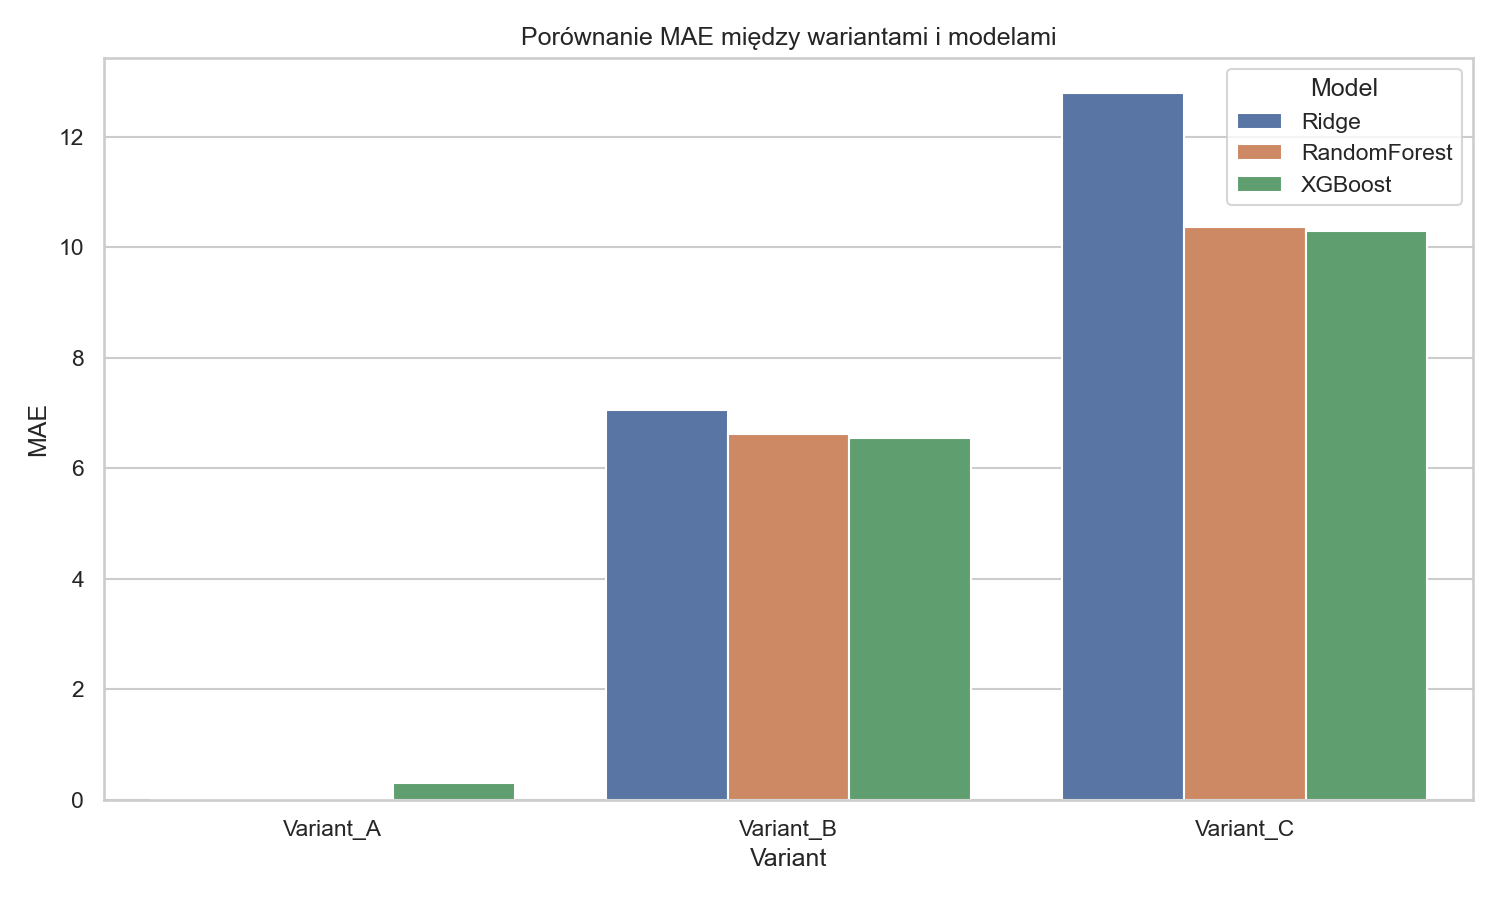
\includegraphics[width=0.9\textwidth]{figures/experiments_partial/mae_comparison.png}
\caption[Porównanie wartości MAE między wariantami i modelami]{Porównanie wartości MAE między wariantami A, B i C oraz modelami Ridge Regression, Random Forest i XGBoost.\par Źródło: Opracowanie własne.}
\label{fig:mae_comparison}
\end{figure}

\begin{figure}[htbp]
\centering
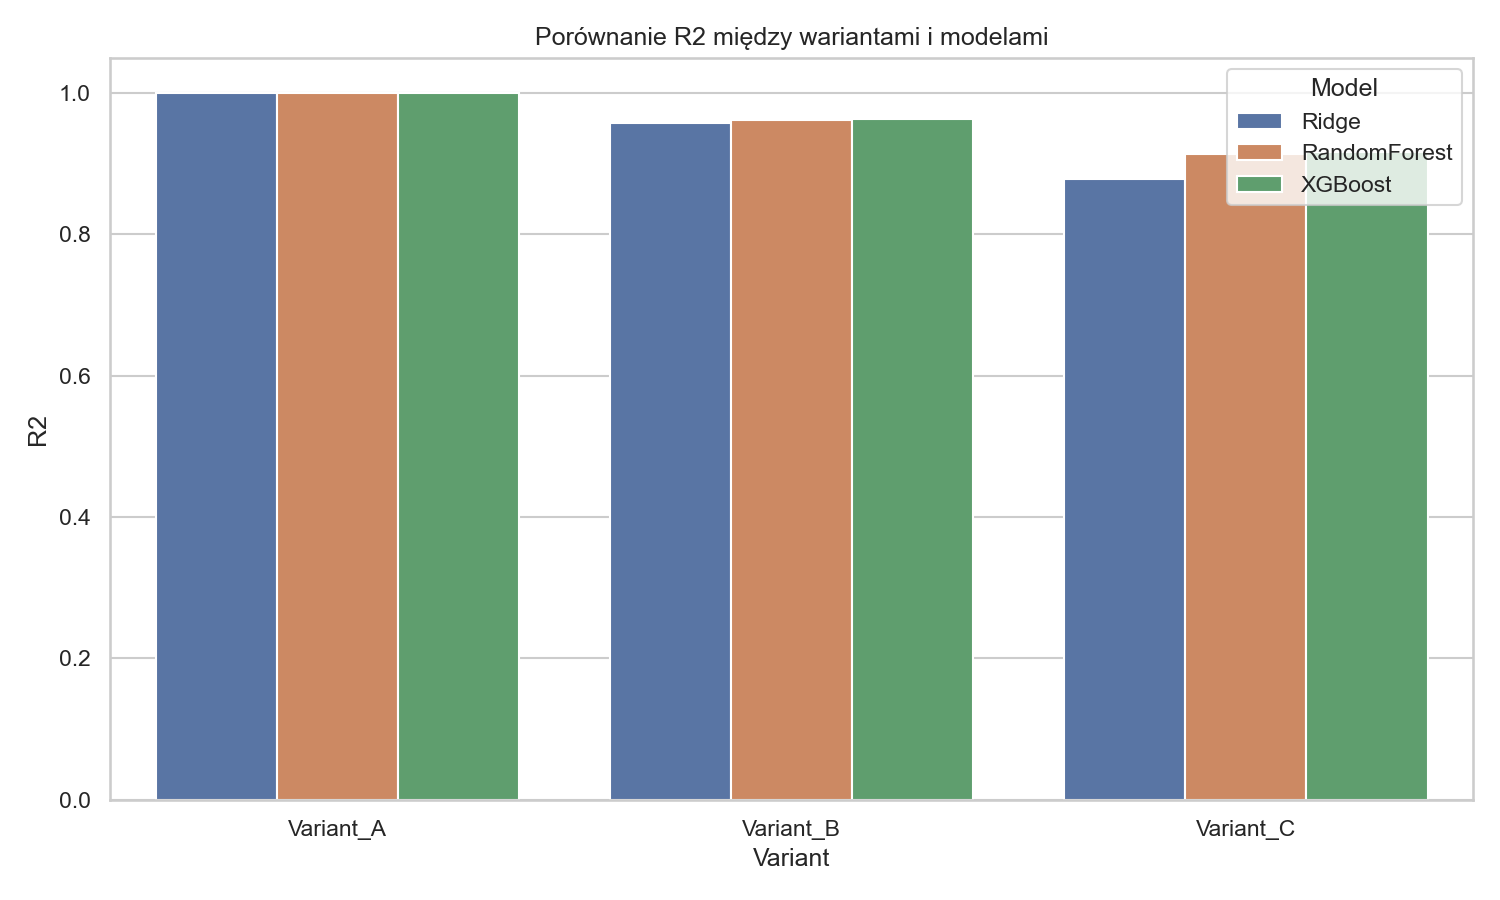
\includegraphics[width=0.9\textwidth]{figures/experiments_partial/r2_comparison.png}
\caption[Porównanie współczynnika R2 między wariantami i modelami]{Porównanie współczynnika determinacji ($R^2$) między wariantami A, B i C oraz modelami Ridge Regression, Random Forest i XGBoost.\par Źródło: Opracowanie własne.}
\label{fig:r2_comparison}
\end{figure}

\FloatBarrier
\section{Analiza rozkładu błędów}

Dla modelu XGBoost w wariancie B przeanalizowano relację pomiędzy wartościami przewidywanymi i referencyjnymi oraz rozkład błędów. Rysunek~\ref{fig:rzeczywiste_vs_przewidywane} pozwala ocenić skupienie predykcji wokół linii idealnego dopasowania, natomiast rysunek~\ref{fig:rozklad_bledow} przedstawia częstotliwość błędów o różnej wielkości.

\begin{figure}[htbp]
\centering
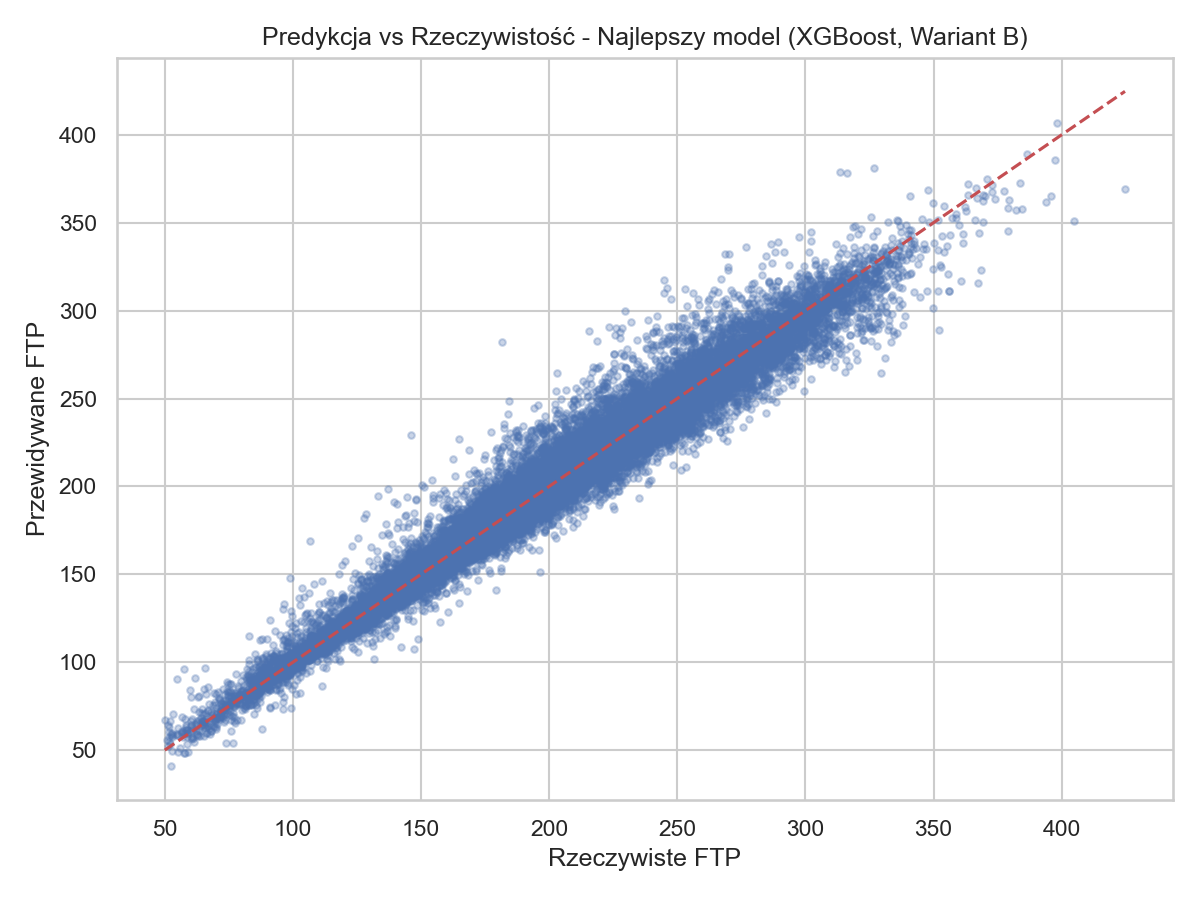
\includegraphics[width=0.9\textwidth]{figures/experiments_partial/pred_vs_actual_best_var_B.png}
\caption[Rzeczywiste i przewidywane wartości FTP dla najlepszego modelu wariantu B]{Zestawienie referencyjnych i przewidywanych wartości FTP dla modelu XGBoost w wariancie B. Linia przerywana oznacza idealne dopasowanie.\par Źródło: Opracowanie własne.}
\label{fig:rzeczywiste_vs_przewidywane}
\end{figure}
\FloatBarrier

Punkty na rysunku~\ref{fig:rzeczywiste_vs_przewidywane} skupiają się wokół linii idealnej predykcji, co jest zgodne z wartościami MAE i $R^2$. Wykres nie zastępuje jednak osobnej analizy błędów dla poszczególnych grup zawodników.

\begin{figure}[htbp]
\centering
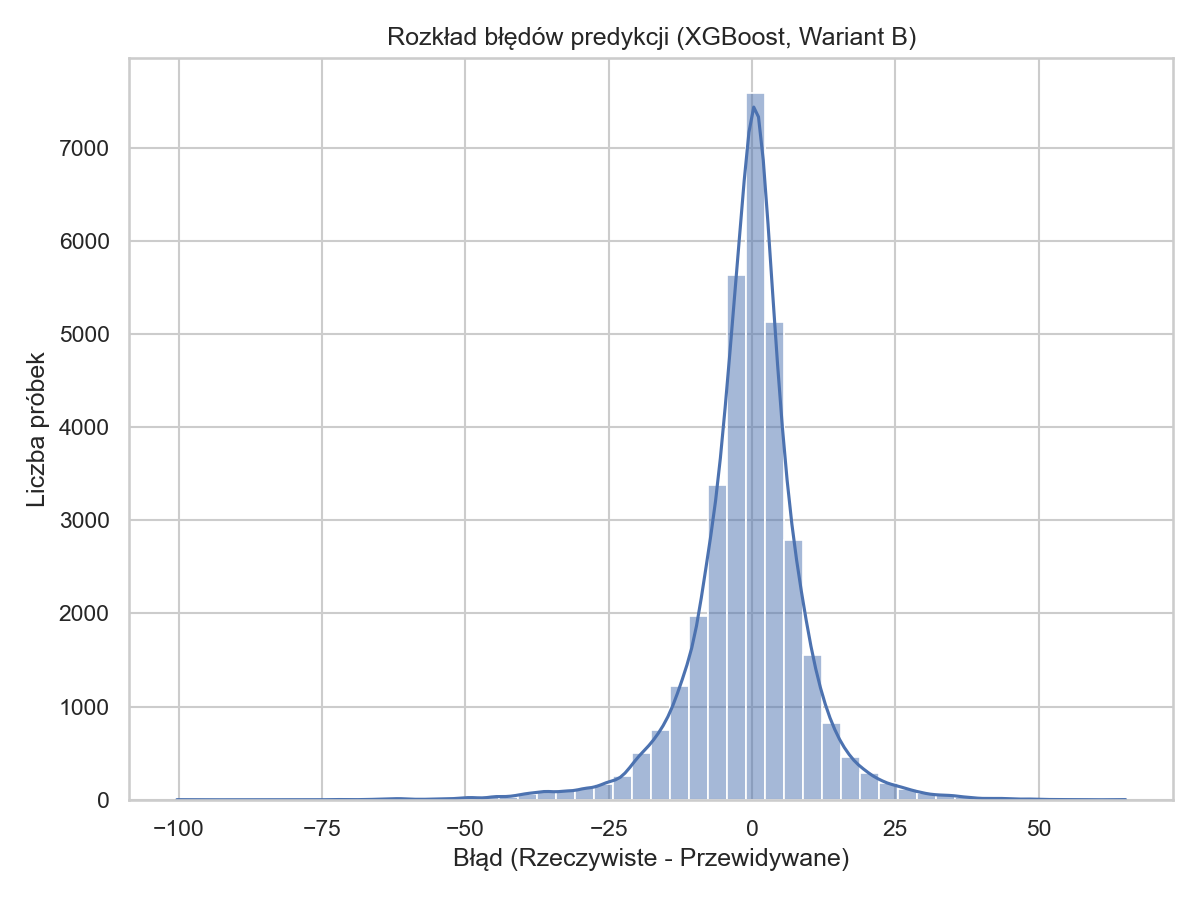
\includegraphics[width=0.9\textwidth]{figures/experiments_partial/error_distribution_best_var_B.png}
\caption[Rozkład błędów najlepszego modelu wariantu B]{Rozkład błędów obliczonych jako wartość referencyjna minus wartość przewidywana dla modelu XGBoost w wariancie B.\par Źródło: Opracowanie własne.}
\label{fig:rozklad_bledow}
\end{figure}
\FloatBarrier

Rozkład błędów na rysunku~\ref{fig:rozklad_bledow} jest skupiony w pobliżu zera. Średni błąd bezwzględny równy 6{,}55 W oznacza, że w historycznym zbiorze testowym typowa różnica pomiędzy etykietą i predykcją była niewielka z perspektywy planowania treningu. Nie oznacza to jednak, że każda pojedyncza prognoza jest obarczona błędem tej samej wielkości.

Histogram błędów uzupełnia wykres predykcji względem etykiety. Pozwala zobaczyć, czy większość różnic koncentruje się blisko zera i czy występują ogony rozkładu związane z trudniejszymi przypadkami. Ponieważ przedstawiona analiza dotyczy wszystkich sesji testowych łącznie, nie wskazuje bezpośrednio, czy większe pomyłki są związane z konkretnym typem treningu, jakością sensora, zakresem FTP albo profilem zawodnika. Takie rozwarstwienie stanowi uzasadniony kierunek dalszej oceny.

\section{Znaczenie i ważność cech predykcyjnych}

Modele drzewiaste umożliwiają analizę względnej ważności cech. Miara ta opisuje wkład predyktorów w decyzje modelu, ale nie pozwala wnioskować o związku przyczynowo-skutkowym. Bardziej szczegółową interpretację lokalnych predykcji można w przyszłości uzupełnić metodą SHAP \parencite{lundberg2017shap}. Rysunki~\ref{fig:waznosc_cech_B} i~\ref{fig:waznosc_cech_C} przedstawiają 20 najważniejszych predyktorów dla modeli XGBoost odpowiednio w wariancie B i C.

Ważność cech należy traktować jako narzędzie diagnostyczne modelu, a nie ranking mechanizmów fizjologicznych. Predyktory mogą być ze sobą skorelowane, przez co informacja przypisana jednej zmiennej mogłaby zostać częściowo przejęta przez inną po zmianie zestawu wejściowego. Wysoka pozycja cechy nie dowodzi również, że jej zmiana wywoła zmianę FTP. Pokazuje jedynie, że algorytm korzystał z niej podczas budowania predykcji w analizowanym zbiorze.

\begin{figure}[htbp]
\centering
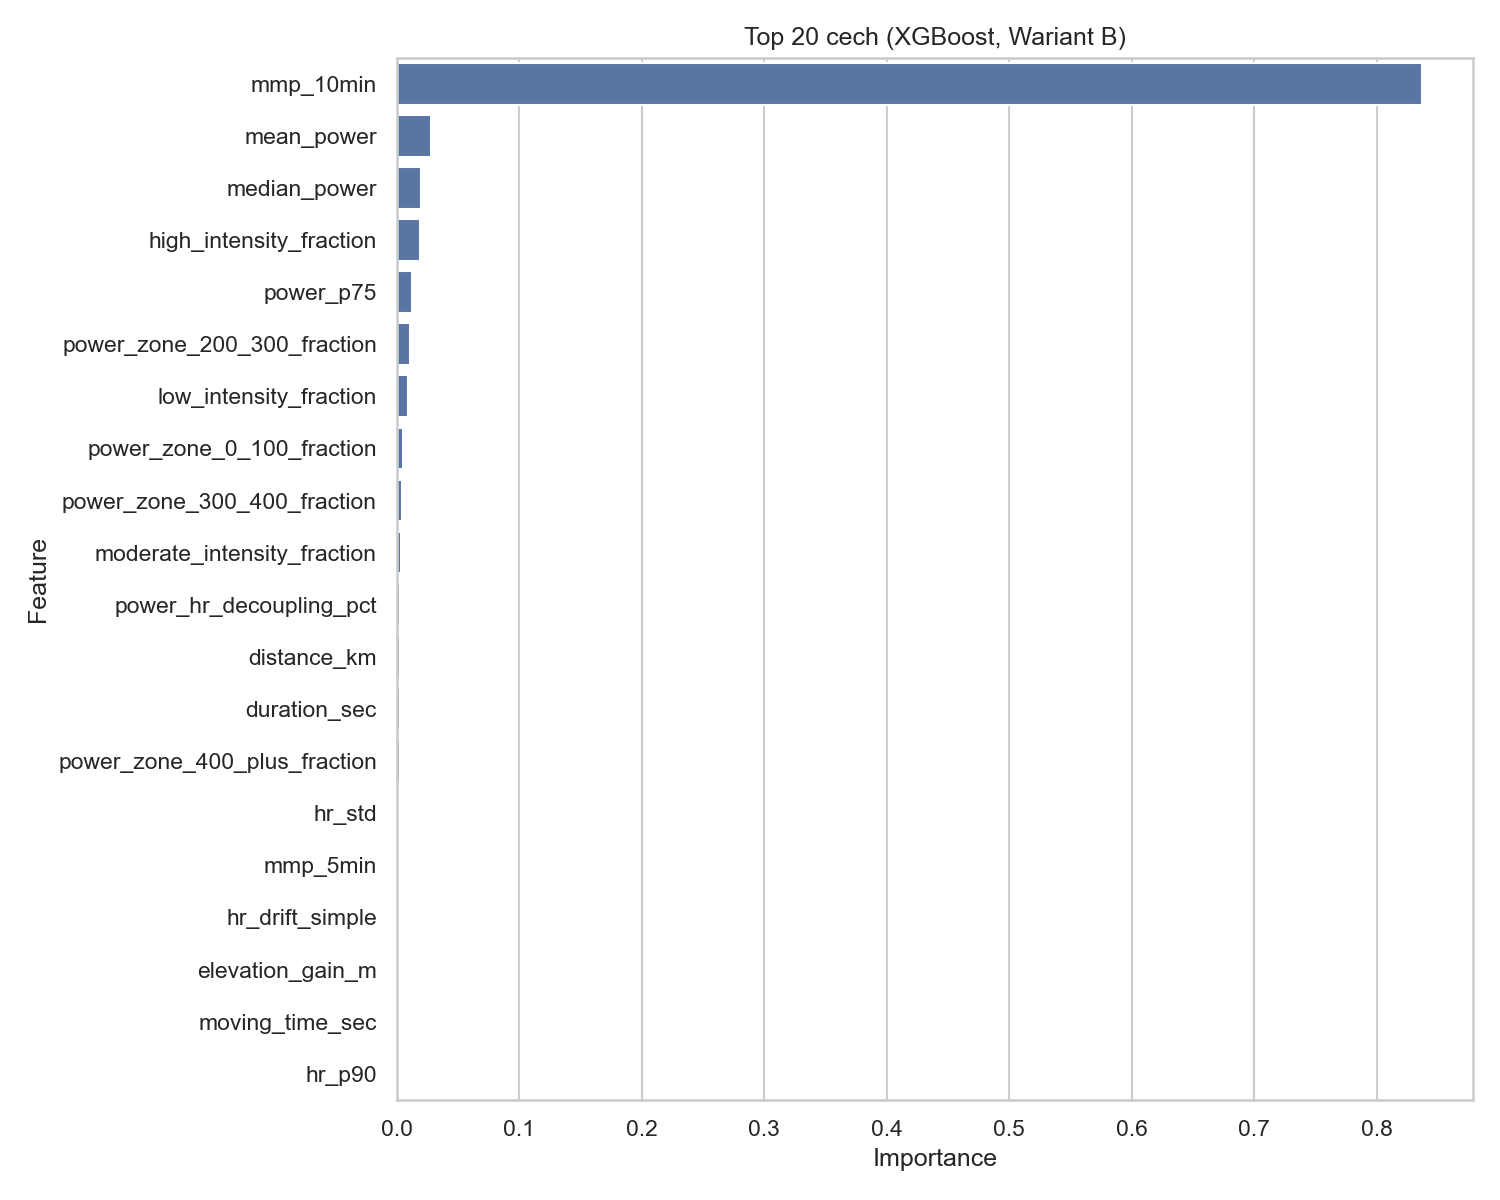
\includegraphics[width=0.9\textwidth]{figures/experiments_partial/feature_importance_best_var_B.png}
\caption[Ważność cech dla modelu XGBoost w wariancie B]{Dwadzieścia najważniejszych predyktorów dla modelu XGBoost w wariancie B.\par Źródło: Opracowanie własne.}
\label{fig:waznosc_cech_B}
\end{figure}

\begin{figure}[htbp]
\centering
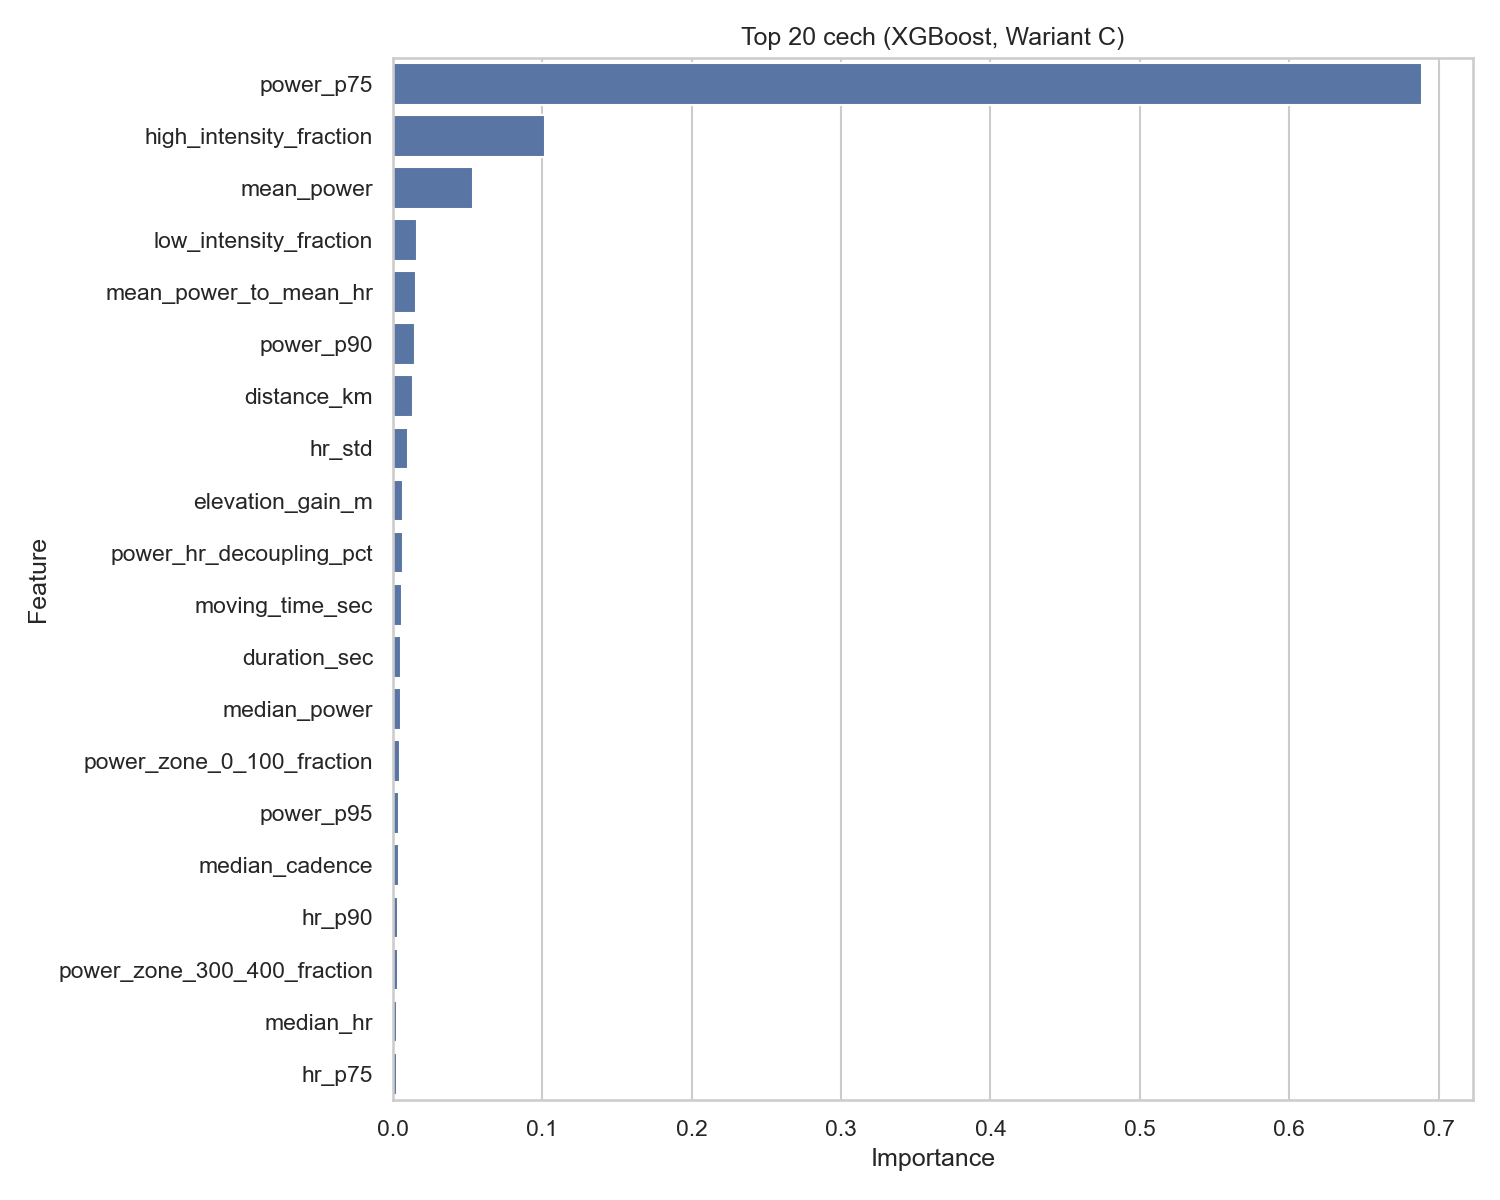
\includegraphics[width=0.9\textwidth]{figures/experiments_partial/feature_importance_best_var_C.png}
\caption[Ważność cech dla modelu XGBoost w wariancie C]{Dwadzieścia najważniejszych predyktorów dla modelu XGBoost w konserwatywnym wariancie C po usunięciu cech z prefiksem \texttt{mmp\_}.\par Źródło: Opracowanie własne.}
\label{fig:waznosc_cech_C}
\end{figure}
\FloatBarrier

W wariancie B dominowała cecha \texttt{mmp\_10min}; znaczenie miały również statystyki mocy oraz cechy opisujące rozkład intensywności. Po usunięciu całej grupy \texttt{mmp\_*} wariant C opierał się w większym stopniu na kwantylach mocy, udziale czasu w strefach intensywności oraz relacji mocy do tętna. Zestawienie wskazuje, że model wykorzystuje kilka grup cech, a nie pojedynczy predyktor.

Zmiana rankingu pomiędzy wariantami B i C jest informacyjna sama w sobie. Po usunięciu cech MMP algorytm nie traci całkowicie zdolności predykcyjnej, lecz przenosi ciężar decyzji na pozostałe podsumowania sesji. Potwierdza to, że dataset zawiera sygnał rozproszony w kilku grupach predyktorów. Jednocześnie nie pozwala rozstrzygnąć, które cechy byłyby najbardziej stabilne w innym repozytorium danych lub w walidacji prospektywnej.

\FloatBarrier
\section{Dodatkowa próba kontrolna skalowalności}

Po zakończeniu eksperymentu bazowego wykonano dodatkową próbę kontrolną na rozszerzonym zbiorze GoldenCheetah OpenData obejmującym 5000 archiwów ZIP. Próba ta nie zastępuje wyników opisanych w poprzednich sekcjach, lecz służy ocenie stabilności potoku oraz sprawdzeniu, czy główne obserwacje utrzymują się przy większej liczbie zawodników. Zachowano tę samą definicję etykiety, filtr FTP, warianty A/B/C, modele oraz podział po \texttt{athlete\_id}.

Po filtracji FTP zbiór kontrolny obejmował 4645 zawodników i 979\,672 sesje treningowe. W wariancie A ponownie uzyskano niemal idealne metryki, co potwierdza, że konfiguracja ta pozostaje obciążona leakage i nie powinna być interpretowana jako właściwy wynik badawczy. W wariancie B najlepszy wynik w próbie kontrolnej uzyskał Random Forest: MAE = 6{,}01 W oraz $R^2 = 0{,}9679$. Wariant C osiągnął niższą jakość, ale nadal zachował wysoką zdolność odtwarzania etykiety FTP.

\begin{table}[htbp]
\centering
\caption{Porównanie skali eksperymentu bazowego i próby kontrolnej}
\label{tab:baseline_control_scale}
\small
\begin{tabular}{|>{\raggedright\arraybackslash}p{4.4cm}|c|c|}
\hline
\textbf{Element} & \textbf{Eksperyment bazowy} & \textbf{Próba kontrolna} \\ \hline
Liczba archiwów ZIP & 781 & 5000 \\ \hline
Liczba zawodników po filtrze FTP & 726 & 4645 \\ \hline
Liczba sesji po filtrze FTP & 151\,399 & 979\,672 \\ \hline
Najlepszy model wariantu B & XGBoost & Random Forest \\ \hline
Najlepsze MAE wariantu B & 6{,}55 W & 6{,}01 W \\ \hline
Najlepsze $R^2$ wariantu B & 0{,}9630 & 0{,}9679 \\ \hline
\end{tabular}
\par\smallskip
\raggedright\footnotesize Źródło: Opracowanie własne na podstawie plików \texttt{results/model\_comparison\_partial.csv} oraz \texttt{experiments/control\_5000/results/control\_5000\_metrics.csv}.
\end{table}

Rysunek~\ref{fig:baseline_vs_control_5000_metrics} porównuje metryki MAE i $R^2$ dla wariantów B i C w eksperymencie bazowym oraz w próbie kontrolnej. Wariant A pominięto na wykresie, ponieważ jego bardzo niskie błędy wynikają z bezpośredniego wycieku informacji z cechy \texttt{mmp\_20min}.

\begin{figure}[htbp]
\centering
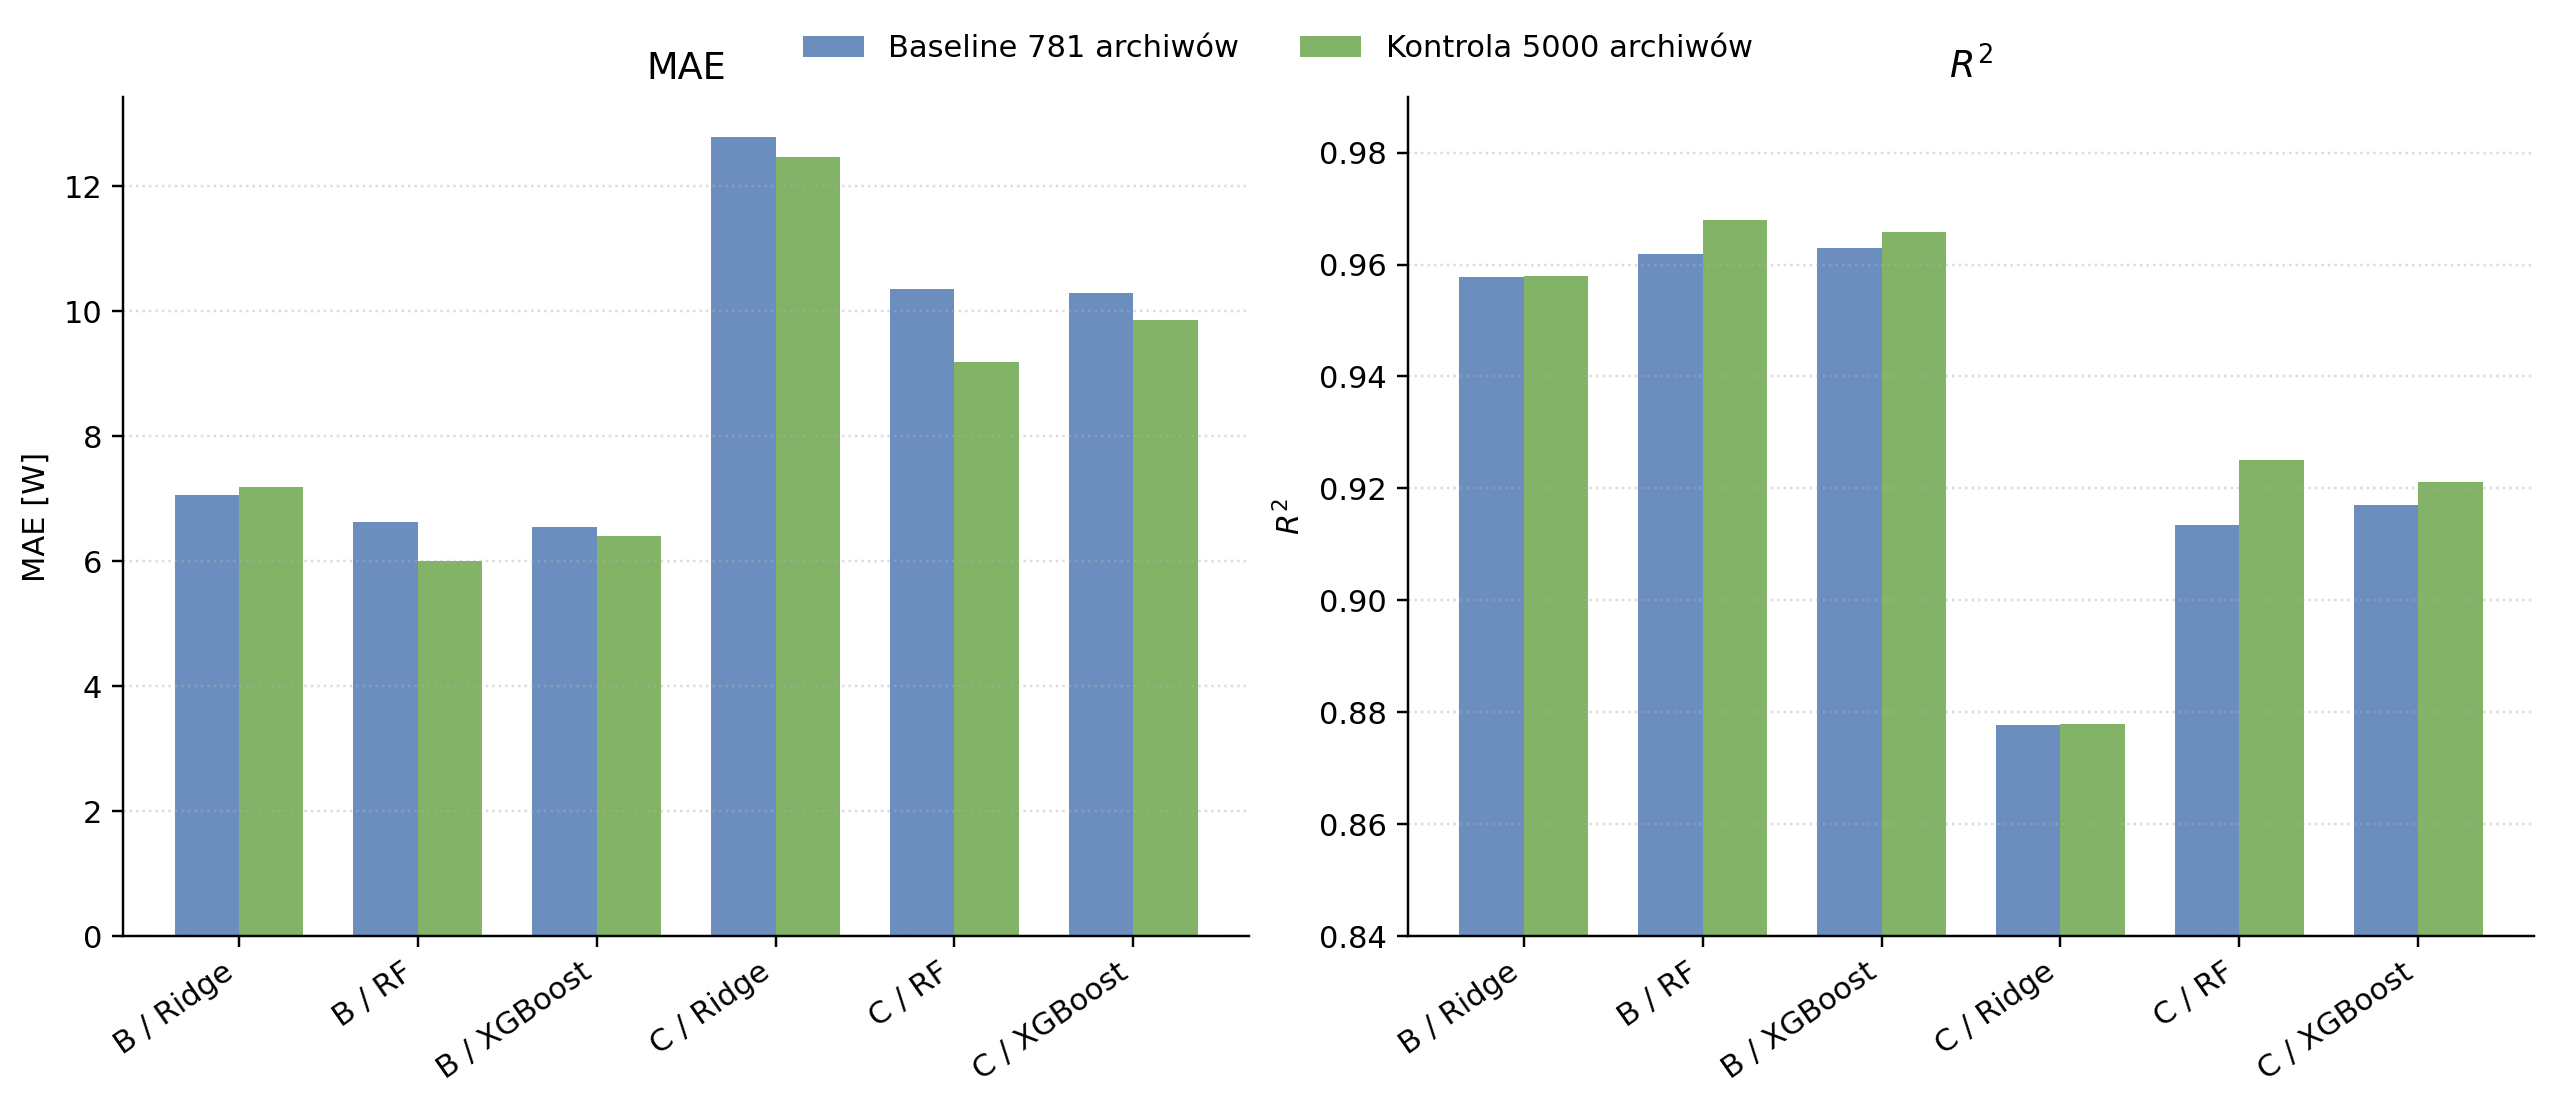
\includegraphics[width=0.98\textwidth]{figures/control_5000/baseline_vs_control_5000_metrics.png}
\caption[Porównanie eksperymentu bazowego i próby kontrolnej 5000 archiwów]{Porównanie wartości MAE i $R^2$ dla wariantów B i C w eksperymencie bazowym oraz w próbie kontrolnej obejmującej 5000 archiwów GoldenCheetah.\par Źródło: Opracowanie własne na podstawie zapisanych wyników eksperymentów.}
\label{fig:baseline_vs_control_5000_metrics}
\end{figure}

Wyniki próby kontrolnej są zgodne z główną interpretacją pracy: usunięcie \texttt{mmp\_20min} ogranicza bezpośredni wyciek, wariant B pozostaje najsilniejszą praktyczną konfiguracją, a wariant C pokazuje koszt bardziej konserwatywnego usunięcia całej grupy cech MMP. Różnice pomiędzy modelami nie zmieniają metodologii ani wniosków bazowego eksperymentu; wskazują jedynie, że potok zachowuje stabilność przy większej skali danych.

\FloatBarrier
\section{Podsumowanie uzyskanych rezultatów}

Celem eksperymentu była ocena jakości pasywnej estymacji FTP oraz identyfikacja wycieku danych. Wariant A potwierdził, że włączenie \texttt{mmp\_20min} prowadzi do sztucznie zawyżonych wyników i nie może stanowić podstawy oceny rozwiązania. W głównym wariancie B najlepszy był XGBoost z MAE = 6{,}55 W i $R^2 = 0{,}9630$. Wariant C, po usunięciu wszystkich cech \texttt{mmp\_*}, uzyskał wyższy błąd, ale nadal pozwalał odtworzyć znaczną część wariancji etykiety FTP.

Podział osobniczy sprawił, że wszystkie modele oceniano na sesjach zawodników nieobecnych w zbiorze treningowym. Ogranicza to ryzyko, że algorytm odtwarza charakterystyczny profil konkretnej osoby zamiast uczyć się relacji możliwych do uogólnienia. Zbliżone rezultaty XGBoost i Random Forest w wariancie B wskazują również, że wysoka jakość predykcji nie zależy wyłącznie od jednego algorytmu.

Wariant C pełni ważną funkcję interpretacyjną. Wzrost MAE z 6{,}55 W do 10{,}29 W pokazuje, że cechy MMP inne niż \texttt{mmp\_20min} niosą istotną informację o wydolności zawodnika. Jednocześnie utrzymanie $R^2 = 0{,}9170$ po ich usunięciu sugeruje, że model może wykorzystywać także rozkład intensywności, kwantyle mocy oraz cechy relacji mocy do tętna.

Błąd wyrażony w watach należy interpretować jako średnią różnicę pomiędzy predykcją a heurystyczną etykietą historyczną. MAE nie wyznacza maksymalnej pomyłki dla pojedynczej sesji i nie potwierdza równoważności z kontrolowanym badaniem laboratoryjnym. Wyniki wskazują jednak, że dane telemetryczne mogą być użyteczne w narzędziu wspomagającym monitorowanie formy. Przed wykorzystaniem rozwiązania w praktyce potrzebna jest walidacja prospektywna.
